\documentclass[a4paper,openany]{uantwerpenassignment}

\usepackage[dutch]{babel}
\usepackage{titlesec}
\usepackage{tikz}
\usepackage{pythonhighlight}
\usepackage{amsmath}
\usepackage{array}

\newenvironment{conditions}
  {\par\vspace{\abovedisplayskip}\noindent\begin{tabular}{>{$}l<{$} @{${}={}$} l}}
  {\end{tabular}\par\vspace{\belowdisplayskip}}

\definecolor{code}{HTML}{ecf0f1}
\definecolor{codetext}{HTML}{d9534f}
\newcommand{\codeword}[1]{
    \colorbox{code}{\texttt{\textcolor{codetext}{#1}}}
}

\newcommand{\reference}[1]{\textit{\ref{#1}. \nameref{#1}}}

\facultyacronym{TI}

\title{\sffamily Chess AI-Agent}
\subtitle{\sffamily5-Artificiële Intelligentie}
\author{\sffamily Mathias Maes, Tijs Van Alphen \\en Willem Van der Elst}

\programme{BA}{IW}{EI}

\academicyear{2020-2021}

\publisher{}

\titleformat{\chapter}{\sffamily\huge\bfseries}{\thechapter.}{10pt}{\sffamily\huge\bfseries}
\titleformat{\section}{\sffamily\LARGE\bfseries}{\thesection.}{10pt}{\sffamily\LARGE\bfseries}
\titleformat{\subsection}{\sffamily\Large\bfseries}{\thesubsection.}{10pt}{\sffamily\Large\bfseries}
\titleformat{\subsubsection}{}{}{10pt}{\sffamily\large\bfseries}


\begin{document}

\sffamily
\maketitle

\tableofcontents

\chapter{Keuze}

Het type AI was een belangrijke keuze van dit project. Het moest haalbaar zijn om te implementeren binnen de beperkte tijdsperiode en we moesten onze eigen niet-supercomputers gebruiken om te treinen. Een lijst  met de voor- en nadelen van de verschillende opties werd opgesteld.


\textbf{Search}:\\
No time to study the whole tree (too much states)

\textbf{Multi-Agent search} (Minimax, Alpha-Beta pruning):\\
Method used by multiple sources, but we have no experience with it. 

\textbf{Reinforcement learning} (Generalised Q learning):\\
We've already used this and therefore we already understand it and can implement it quickly.\\
Once trained, it will act optimally. The training however, needs a lot of time to learn and the choice of features isn't that obvious.

\textbf{Neural network/ Deep learning:}
- No data labels
- Never Done
- No clue of in/output


Q-Learning leek ons het interessantst, maar Minimax was haalbaarder en zou sowieso een goed resultaat leveren. We besloten om beide methodes uit te werken. 

Uiteindelijk ging de keuze naar beide agents. We hadden namelijk een thesis\cite{rl} gevonden die een minimax agent gebruikte als feature voor een generalized Q-Learner.

\chapter{Alpha-Beta Pruning}

\section{Utility}
\label{utility}

Onze utility maakt gebruik van veel kenmerken van de features van onze Q-Learner dus gaan we dit later behandelen.
Je kan op het moment onze utility als volgt begrijpen:

$$
u(S) = 
\begin{cases}
    100 &\mbox{Als je gewonnen hebt}\\
    -30 &\mbox{Als er een stalemate gespeeld is}\\
    -100 &\mbox{Als je verloren hebt}\\
    c + C + \Delta M + \Delta m + s + f_q &\mbox{Bij overige situaties}
\end{cases}
$$

\begin{conditions}
    c & Of er gecastled is met de vorige move\\
    C & Of het bord in schaak staat\\
    \Delta M & Het materiaal verschil op het bord\\
    \Delta m & Het verschil in mobility\\
    s & De positie score voor alle eigen stukken\\
    f_q & Een gewogen(geleerd of niet-geleerd) aantal features
\end{conditions}

Hoe deze kleine sub-functies bepaald worden wordt later nog besproken in het stuk \reference{features}.

\chapter{Q-Learning Agent}

\section{Generalization}

De eerste agent die we moesten maken was de Q-agent deze is generalized omdat zoals bij de minpunten stonden van general search algoritmes, is het bijna onmogelijk om elke staat te bezoeken. Daarom dat we niet gewoon Q-learning gaan doen maar generalized Q-learning.

\section{Features}
\label{features}

We hebben een hoop features gedefinieerd deze zijn voornamelijk gebaseerd op de paper\cite{rl} die we gevonden hebben. De bedoeling van deze features is om een state zo goed mogelijk te definiëren. Je kan hieronder een beschrijving vinden van elks van onze 55 features.

We berekenen onze features als volt:

$$
Q(s,a) = \sum_{i} w_{i} \cdot \sigma \left( f_i(s, a)\right)
$$

De $\sigma(x)$ die we in de berekening zien wordt als volgt gedefinieerd:

$$
\sigma(x) = \frac{2}{1 + e^{-x}} - 1
$$

Dit is een aangepaste versie van de bekende sigmoid\cite{WSF} functie. Onze versie zorgt in tegenstelling tot de originele er voor dat waardes in het interval $\left]-1,1\right[$ vallen.\\
Hier zie je de grafiek van de functie:

\begin{figure}[h]
    \centering
    \begin{tikzpicture}[scale=2]
        \draw[->] (-2, 0) -- (2, 0) node[right] {$x$};
        \draw[->] (0, -1.2) -- (0, 1.2) node[above] {$y$};

        \draw[dashed] (-2, 0.5) -- (2, 0.5);
        \node (A) at (-2, 0.6) {\tiny $1$};

        \draw[dashed] (-2, -0.5) -- (2, -0.5);
        \node (B) at (-2, -0.6) {\tiny $-1$};

        \draw[scale=0.5, domain=-3.9:3.9, smooth, variable=\x, blue] plot ({\x}, { 2/(1 + exp(-\x)) - 1 });
        \node[blue] (C) at (0.4, 0.32) {$\sigma$};
    \end{tikzpicture}
    \caption{$\sigma(x)$} \label{fig:sigmoid}
\end{figure}


\subsection{Material}
\subsection{Mobility}
\subsection{Attackers}
\subsection{Forks}
\subsection{Control}
\subsubsection{Center Control}
\subsubsection{Board Control}

\section{Reward}


Evaluation\cite{chessprogramming}

\chapter{Optimalisaties}

We hebben een hoop optimalisaties moeten toevoegen aan onze Q-Learner om hem zo rap mogelijk te laten denken.

\section{Multi-Threading}

We hebben multi-threading toegevoegd aan onze q-learner zo berekent hij de q-waarde van elke actie in een aparte thread. We hebben bewust niet gekozen om elke feature apart omdat dit onze timing issues verergerde in plaat van verbeterde.

We hebben door multi-threading onze iteratie tijd met 20\% weten dalen.

Hier zie je de resultaten van het processor gebruik:

\begin{figure}[h]
    \centering
    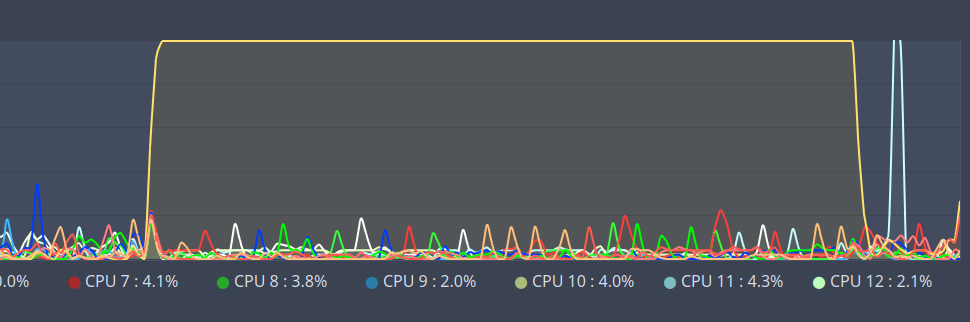
\includegraphics[width=300pt]{images/singlethreaded.png}
    \caption{Single Threaded Q-Learner CPU usage}
    \label{fig:singlethreaded}
\end{figure}

\begin{figure}[h]
    \centering
    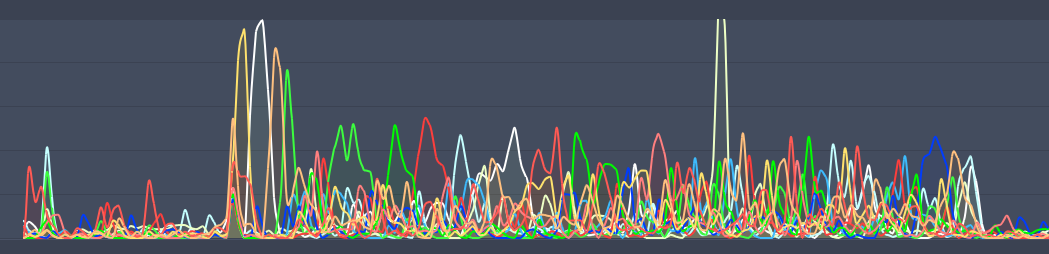
\includegraphics[width=350pt]{images/multithreaded.png}
    \caption{Multi Threaded Q-Learner CPU usage}
    \label{fig:multithreaded}
\end{figure}

\section{Caching}

We gebruiken ook veel plaatsen caching zodat we niet 2 keer hetzelfde moeten uitrekenen. De meest bijzondere cache is deze voor onze alpha-beta feature, deze moet per bord state maar 1 keer uitvoeren waardoor we de alpha-beta langer kunnen laten zoeken en een hoop tijd besparen.
Det tijd die we hierdoor besparen per iteratie kan soms tot een minuut of 2 oplopen.

\chapter{Resultaten}
\section{GrandQ vs. Stockfish (0-544)}

Command:\\
\codeword{python3 train -o stockfish --skill 0 --depth 10 -tt 5 -dt 0 -e 0.3 -d 0.6 -l 0.01 -q -i -1}

\section{GrandQ vs. Alpha-Beta (544 - 5732)}

Command:\\
\codeword{python3 train -o ab --depth 10 -tt 5 -dt 0 -e 0.3 -d 0.6 -l 0.01 -q -i -1}

Command na ongveer 1500 episodes:\\
\codeword{python3 train -o ab --depth 10 -tt 5 -dt 0 -e 0.2 -d 0.4 -l 0.01 -q -i -1}

\bibliography{sources}
\bibliographystyle{ieeetr}

\end{document}
